%%------------------------------------------------------------------------------
%%Präambel laden
%%------------------------------------------------------------------------------
%%------------------------------------------------------------------------------
%%Klasse
%%------------------------------------------------------------------------------
\documentclass[a5paper,landscape,DIV=calc,11pt,notitlepage]{scrartcl}
%%------------------------------------------------------------------------------
%%Packages
%%------------------------------------------------------------------------------
\usepackage[headsepline=no, footsepline=no]{scrlayer-scrpage}
\usepackage[utf8]{inputenc}
\usepackage[T1]{fontenc}
\usepackage{CJKutf8}
\usepackage[ngerman]{babel} 
\usepackage[left=24pt, right=24pt, top=24pt, bottom=24pt]{geometry}
\usepackage{tabularx}
\usepackage[svgnames,RGB,table]{xcolor}
\usepackage{booktabs}
\usepackage{multicol,multirow}
\usepackage[lining]{libertinus}	%Schriftart -> Libertine, ausgerichtete Ziffern
%\usepackage[oldstyle]{libertinus}	%Schriftart -> Libertine, Minuskeln
%\usepackage[sfdefault]{noto}		%Schriftart -> Noto Sans, -> Schriftgröße auf 10pt runter!
%\usepackage[osf]{libertine}
\usepackage{microtype}
\usepackage[german]{layout}
\usepackage{calc}
\usepackage{float}
\usepackage{tikz}
\usepackage{tcolorbox}
\tcbuselibrary{raster,skins}
\usepackage{layout}
\usepackage{eso-pic}
\usepackage{graphicx}
\usepackage{amssymb}
\usepackage{amsmath}
\usepackage{setspace}
\usepackage{mwe}
\usepackage[pdftex,pdfauthor={Sascha Christmann},pdftitle={G\={o}j\={u}-Ry\={u} Karate-D\={o} Reusrath - Trainigskarten},pdfproducer={MiKTeX},pdfcreator={pdflatex}]{hyperref}
\usepackage{datetime}
\usepackage{import}
%%------------------------------------------------------------------------------
%%Vereinbarungen & Makros
%%------------------------------------------------------------------------------
\clearpairofpagestyles
\newcounter{num}
\newcounter{numz}
\newcommand{\ctu}[0]{\stepcounter{num}\arabic{num}.}
\newcommand{\ctuz}[0]{\stepcounter{numz}\arabic{numz}}
\newcommand{\ctd}[0]{\addtocounter{num}{-1}\arabic{num}.}
\newcommand{\ctdz}[0]{\addtocounter{numz}{-1}\arabic{numz}}	
\setcounter{num}{0}
\setcounter{numz}{0}
%%------------------------------------------------------------------------------
\newlength\tindent
\setlength{\tindent}{\parindent}
\setlength{\parindent}{0pt}
\renewcommand{\indent}{\hspace*{\tindent}}
%%------------------------------------------------------------------------------
\graphicspath{{Gfx/gkd/}{Gfx/habersetzer/}{Gfx/gurte/}{Gfx/sglgrkr/}{Gfx/self/}{Gfx/yuishinkan_kamen/}}
%%------------------------------------------------------------------------------
\definecolor{GKD}{rgb}{0.53,0.086,0.102}
\definecolor{SGL}{rgb}{0,0.580,0.290}
\definecolor{SGL2}{rgb}{0,1,0}
\definecolor{YBELT}{rgb}{1,1,0.2}
\definecolor{OBELT}{rgb}{1,0.404,0}
\definecolor{GBELT}{rgb}{0.431,0.686,0.282}
\definecolor{BLBELT}{rgb}{0,0.408,1}
\definecolor{BRBELT}{rgb}{0.376,0.22,0.075}
\definecolor{BKBELT}{rgb}{0.078,0.071,0.071}
%%------------------------------------------------------------------------------
\let\svthefootnote\thefootnote
\newcommand\freefootnote[1]{\let\thefootnote\relax\footnotetext{#1}\let\thefootnote\svthefootnote}
%%------------------------------------------------------------------------------
\newcommand{\trenner}[1]{\vspace{{#1}pt}\hrule\relax\vspace{{#1}pt}}
%%------------------------------------------------------------------------------
\newlength{\VTL}
\newcommand{\SETVTL}[1]{\settowidth{\VTL}{{#1}}}
%%------------------------------------------------------------------------------
\newcommand\ShowBelt[1]{\put(248,-188){\parbox[b][\paperheight]{\paperwidth}{\vfill\centering\includegraphics[width=48pt,keepaspectratio]{#1}\vfill}}}
%%------------------------------------------------------------------------------
\newcommand\ShowLogo{\put(-248,-188){\parbox[b][\paperheight]{\paperwidth}{\vfill\centering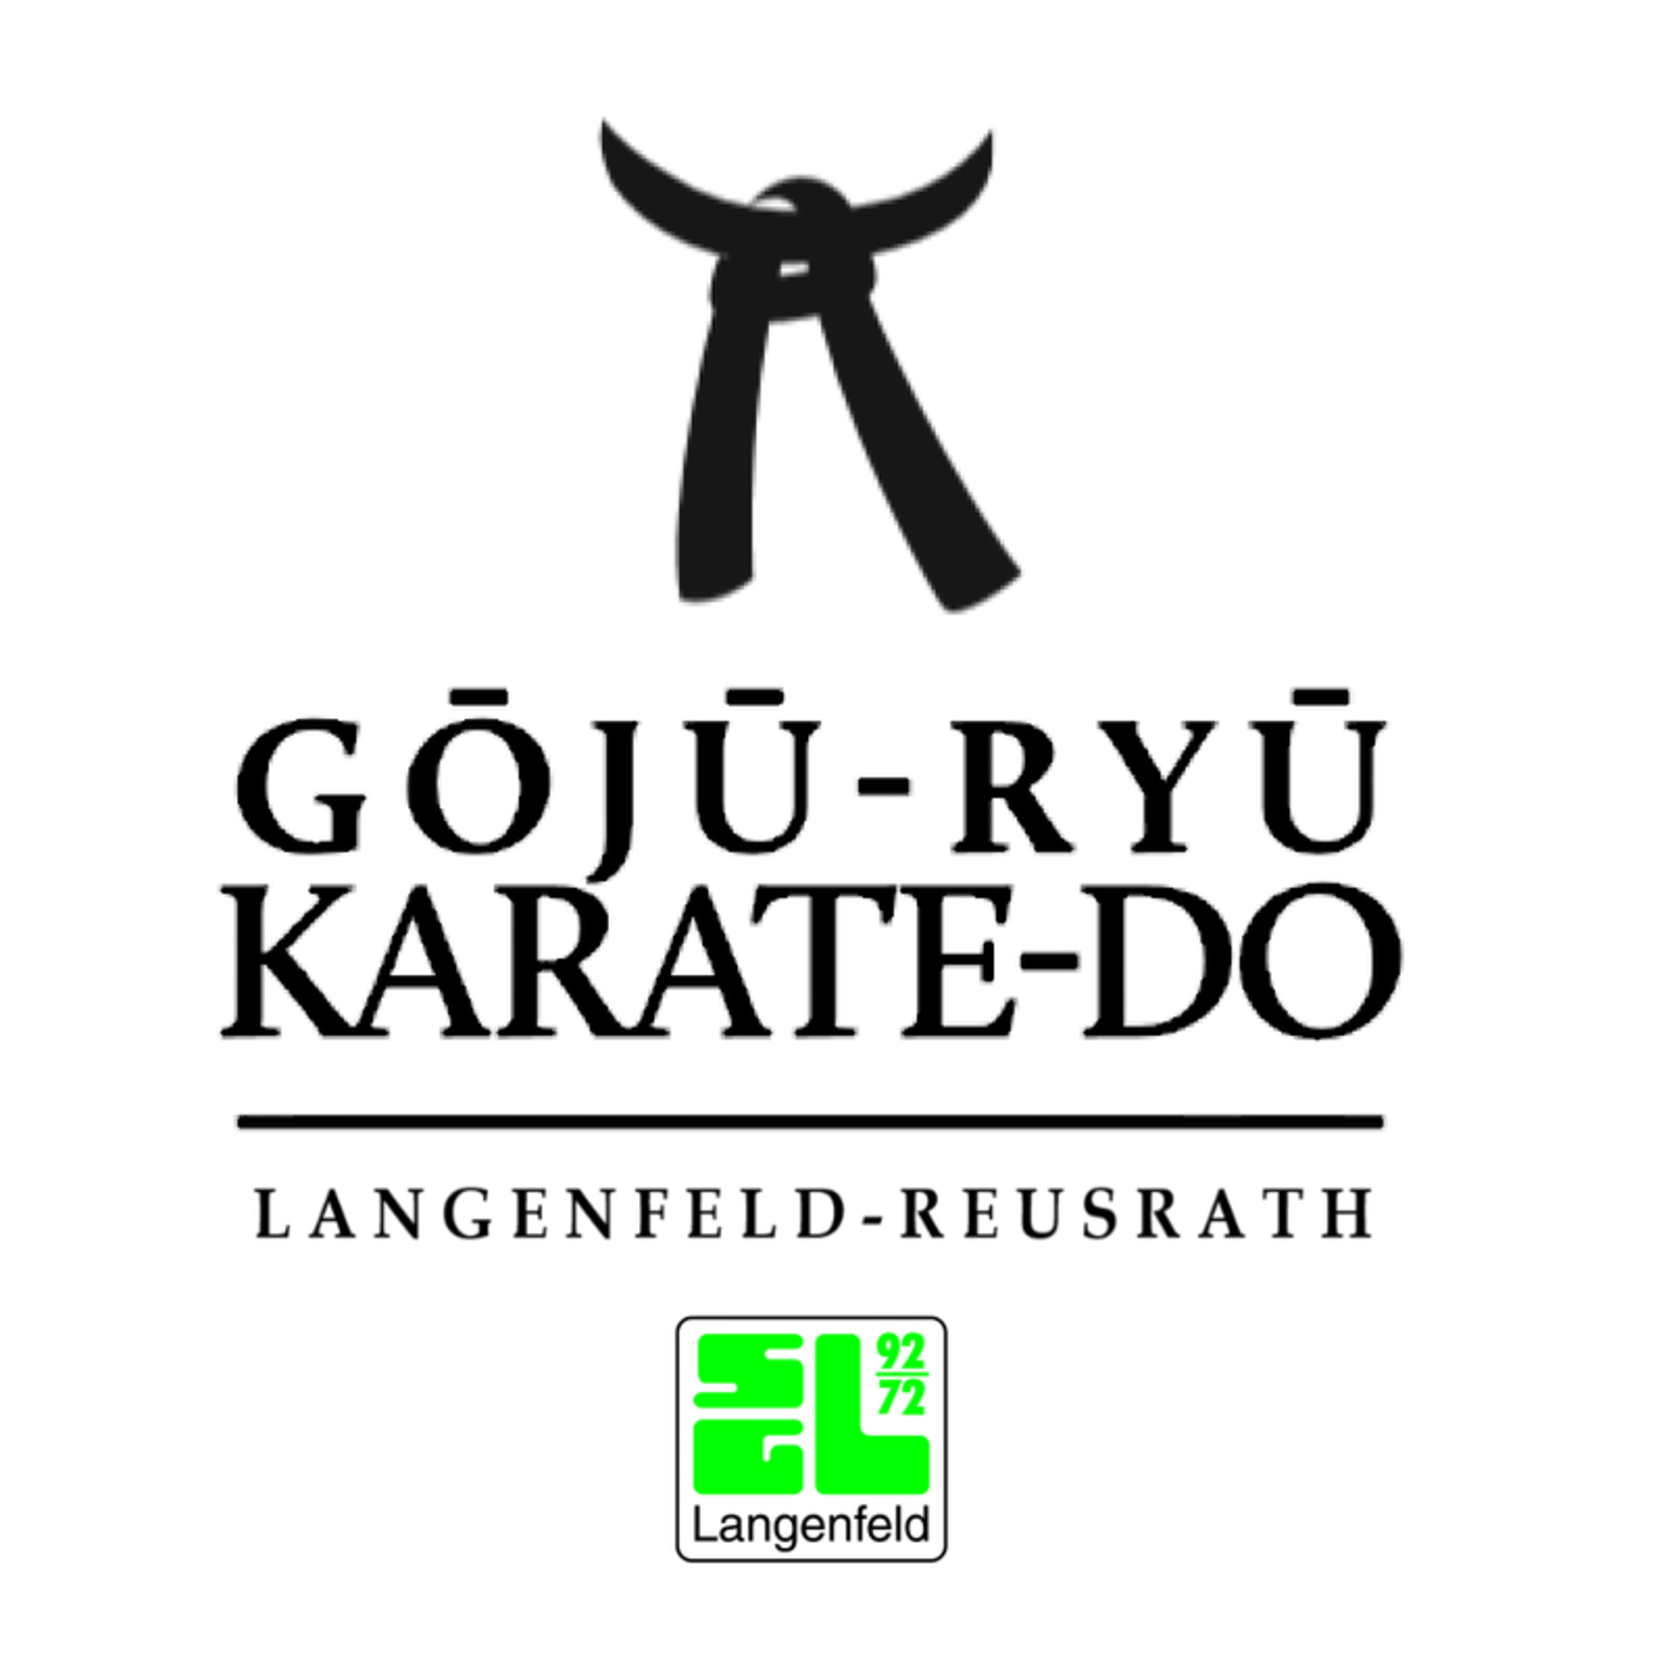
\includegraphics[width=48pt,keepaspectratio]{GJRKDR_n.pdf}\vfill}}}
%%------------------------------------------------------------------------------
\newcommand\ShowDraft{\put(-256,172){\parbox[b][\paperheight]{\paperwidth}{\vfill\centering
\includegraphics[width=72pt,keepaspectratio]{entwurf.pdf}\vfill}}}
%%------------------------------------------------------------------------------
\tcbset{width=\textwidth,height=\textheight,right=12pt,left=12pt,fonttitle=\bfseries}
\newtcolorbox{pfbox}{natural height,leftrule=9pt,rightrule=9pt,right=4pt,left=4pt,colback=white,colframe=GKD}
%%------------------------------------------------------------------------------
%\newenvironment{KANJI}{\CJKfamily{ipxm}\CJKtilde\CJKnospace}{}
%%------------------------------------------------------------------------------
%%EOF
%%------------------------------------------------------------------------------
%%------------------------------------------------------------------------------
%%Ende Präambel
%%------------------------------------------------------------------------------
\begin{document}
%%------------------------------------------------------------------------------
		\null\vfill\null
	{\small 	\begin{tabularx}{\textwidth}{llllX}
			\textbf{Stufe} 	& \textbf{Angriff} 	& \textbf{Block}&\textbf{Konter}&Anmerkung\\
			\midrule
			J\={o}dan 	& Oi-Zuki 	& Age-Uke			&Gyaku-Zuki	& Angriff rechts, Block links, Konter rechts Ch\={u}dan \\
			J\={o}dan 	& Oi-Zuki 	& Age-Uke			&Gyaku-Zuki	& Angriff rechts, Block rechts, Konter links Ch\={u}dan \\	
			Ch\={u}dan	& Oi-Zuki	& Yoko-Uke			&Gyaku-Zuki	& Angriff rechts, Block links, Konter rechts Ch\={u}dan \\
			Ch\={u}dan	& Oi-Zuki	& Soto-Uke			&Gyaku-Zuki	& Angriff rechts, Block links, Konter rechts Ch\={u}dan \\
			Ch\={u}dan	& Ura-Zuki	& Soto-Uke			&Gyaku-Zuki	& Angriff rechts, Block links, Konter rechts J\={o}dan \\
			Ch\={u}dan	& Oi-Zuki	& Shuto-Uke			&Gyaku-Zuki	& Angriff rechts, Block links, Konter rechts \\
			Ch\={u}dan	& Oi-Zuki	& Shuto-Uke			&Gyaku-Zuki	& Angriff rechts, Block rechts, Konter links \\
			Gedan		& Oi-Zuki	& Harai-Otoshi-Uke	&Gyaku-Zuki	& Angriff rechts, Block links, Konter rechts  \\
			Gedan		& Mae-Geri	& Harai-Otoshi-Uke	&Gyaku-Zuki	& Angriff rechts, Block links, Konter rechts \\
			Gedan		& Mae-Geri	& Nagashi-Uke		&Gyaku-Zuki	& Angriff rechts, Block links (rechts), Konter rechts (links)\\
			\midrule
	\end{tabularx}}\null\vfill\null
	\begin{center}
		\begin{minipage}[t]{\textwidth-2\tabcolsep}
			{\footnotesize Als grundlegende Partnerformen der Unterstufe sollten die Techniken mit, dem jeweiligen Können entsprechender, Geschwindigkeit und Definition gezeigt werden. Stete Übung bringt Schnelligkeit. Zu beachten sind die richtige Distanz zum Partner und die korrekte Reaktion auf wechselnde Abstände - Kontertechniken mit Kime setzen. Die Basisübungen sind in der Form \textit{Gerader Angriff - Gerader Konter} beschrieben, sollten aber auch in den Sh\={o}t\={o}kan Varianten mit jeweils 45°-Ausweichbewegungen geübt werden. Dann sind kleinere Anpassungen notwendig, bzw.\,möglich, die sich aus dem Übungsansatz ergeben. Kontertechniken können, und dürfen, entsprechend dem jeweiligen Leistungsstand variiert werden.}\onehalfspacing\singlespacing
			{\footnotesize Die Partnerformen können als \textbf{\textit{Drill}} geübt werden, indem Tori 10 Techniken mit Vorwärtsbewegung ausführt. Am Ende dann Wechsel von Tori zu Uke und 10 Techniken in die andere Richtung. Bei der Ausführung als Drill ist der stetige Seitenwechsel zu beachten, sowie das jeweilig \textquotedblleft richtige Hikite ziehen\textquotedblright. Im Drill bietet es sich an, den Stand auf Sanchin-Dachi zu verkürzen, bzw. für \textit{Gedan Oi-Zuki} auf Shiko-Dachi zu verlängern.}
		\end{minipage}
	\end{center}\null\vfill\null
		\setcounter{num}{0}
\setcounter{numz}{0}
\begin{tcbitemize}[right=4pt,left=4pt,raster columns=3,raster equal height,colframe=GKD,colback=white,fonttitle=\bfseries]
	%%------------------------------------------------------------------------------
	\tcbitem[squeezed title*={Kumite Ura 1}]
	Oi-Zuki Ch\={u}dan
	\trenner{8}
	Tai-Sabaki Hidari 45°\\
	Shisai no Mawashi Geri\,\(\odot\)
	\trenner{8}
	Teish\={o}-Uke\\
	J\={o}dan Ura-Zuki\,\(\odot\)
	%%------------------------------------------------------------------------------
	\tcbitem[squeezed title*={Kumite Ura 2}]
	Oi-Zuki Ch\={u}dan
	\trenner{8}
	Tai-Sabaki Hidari 45°\\
	Yoko-Uke - Uraken-Uchi\,\(\odot\)
	\trenner{8}
	Empi-Uke\\
	J\={o}dan Ura-Zuki\,\(\odot\)
	%%------------------------------------------------------------------------------
	\tcbitem[squeezed title*={Kumite Ura 3}]
	2\,x\,Oi-Zuki Ch\={u}dan
	\trenner{8}
	2\,x\,Yoko-Uke\\
	Mae-Geri\,\(\odot\)
	\trenner{8}
	Teish\={o}-Uke\\
	J\={o}dan Ura-Zuki\,\(\odot\)
\end{tcbitemize}
\null\vfill\null
\begin{pfbox}
	Tori greift vorgehend aus Sanchin-Dachi an. Zu beachten sind gutes Distanzverhalten von Tori und Uke, die erkennbare Ernsthaftigkeit von Angriff und Konter sowie ein runder Ablauf.
\end{pfbox}
\null\vfill\null
\begin{tcbitemize}[right=4pt,left=4pt,raster columns=3,raster equal height,colframe=GKD,colback=white,fonttitle=\bfseries]
	%%------------------------------------------------------------------------------
	\tcbitem[squeezed title*={Kumite Ura 4}]
	Oi-Zuki Ch\={u}dan
	\trenner{8}
	\(\circlearrowleft\)\,90° - Nagashi Technik\\
	J\={o}dan Uraken-Uchi\,\(\odot\)
	\trenner{8}
	Kansetsu-Geri\,\(\odot\)\\
	Suri-Ashi Gedan-Barai\,\(\odot\)
	%%------------------------------------------------------------------------------
	\tcbitem[squeezed title*={Kumite Ura 5}]
	Oi-Zuki Ch\={u}dan
	\trenner{8}
	Ushiro Tai-Sabaki Teish\={o}-Uke\\
	Suri-Ashi J\={o}dan Uraken-Uchi\,\(\odot\)
	\trenner{8}
	Age-Uke\\
	J\={o}dan Ura-Zuki\,\(\odot\)
	%%------------------------------------------------------------------------------
	\tcbitem[squeezed title*={Kumite Ura 6}]
	Oi-Zuki Ch\={u}dan
	\trenner{8}
	Tai-Sabaki Hidari 45° Teish\={o}-Uchi\\
	Furi-Uchi-Ken\,\(\odot\)
	\trenner{8}
	Age-Uke\\
	J\={o}dan Ura-Zuki\,\(\odot\)
	%%------------------------------------------------------------------------------
\end{tcbitemize}
%%------------------------------------------------------------------------------
\clearpage
\newpage
%	\null\vfill\null
\begin{tcbitemize}[right=4pt,left=4pt,raster columns=3,raster equal height,colframe=GKD,colback=white,fonttitle=\bfseries]
	%%------------------------------------------------------------------------------
	\tcbitem[squeezed title*={Kumite Ura 7}]
	Oi-Zuki Ch\={u}dan
	\trenner{8}
	Tai-Sabaki Hidari 45° Teish\={o}-Uchi\\
	J\={o}dan Ura-Zuki\,\(\odot\)
	\trenner{8}
	Eindrehen mit J\={o}dan Nagashi-Uke\\
	Ch\={u}dan Gyaku-Kagi-Zuki\,\(\odot\)
	%%------------------------------------------------------------------------------
	\tcbitem[squeezed title*={Kumite Ura 8}]
	Oi-Zuki Ch\={u}dan
	\trenner{8}
	Ushiro Tai-Sabaki Osae-Uke\\
	Suri-Ashi J\={o}dan Teish\={o}-Uchi\,\(\odot\)
	\trenner{8}
	Yoko-Uke \\
	Uraken-Uchi J\={o}dan\,\(\odot\)
	%%------------------------------------------------------------------------------
	\tcbitem[squeezed title*={Kumite Ura 9}]
	Oi-Zuki Ch\={u}dan
	\trenner{8}
	\textcolor{lightgray}{ergänzen}\\
	\textcolor{lightgray}{ergänzen}
	\trenner{8}
	\textcolor{lightgray}{ergänzen}\\
	\textcolor{lightgray}{ergänzen}
\end{tcbitemize}
\null\vfill\null
\begin{pfbox}
	Tori greift vorgehend aus Sanchin-Dachi an. Zu beachten sind gutes Distanzverhalten von Tori und Uke, die erkennbare Ernsthaftigkeit von Angriff und Konter sowie ein runder Ablauf.
\end{pfbox}
\null\vfill\null
\begin{tcbitemize}[right=4pt,left=4pt,raster columns=3,raster equal height,colframe=GKD,colback=white,fonttitle=\bfseries]
	%%------------------------------------------------------------------------------
	\tcbitem[squeezed title*={Kumite Ura 10}]
	Oi-Zuki Ch\={u}dan
	\trenner{8}
	\textcolor{lightgray}{ergänzen}\\
	\textcolor{lightgray}{ergänzen}
	\trenner{8}
	\textcolor{lightgray}{ergänzen}\\
	\textcolor{lightgray}{ergänzen}
	%%------------------------------------------------------------------------------
	\tcbitem[squeezed title*={Kumite Ura 11}]
	Oi-Zuki Ch\={u}dan
	\trenner{8}
	\textcolor{lightgray}{ergänzen}\\
	\textcolor{lightgray}{ergänzen}
	\trenner{8}
	\textcolor{lightgray}{ergänzen}\\
	\textcolor{lightgray}{ergänzen}
	%%------------------------------------------------------------------------------
	\tcbitem[squeezed title*={Kumite Ura 12}]
	Oi-Zuki Ch\={u}dan
	\trenner{8}
	\textcolor{lightgray}{ergänzen}\\
	\textcolor{lightgray}{ergänzen}
	\trenner{8}
	\textcolor{lightgray}{ergänzen}\\
	\textcolor{lightgray}{ergänzen}
	%%------------------------------------------------------------------------------
\end{tcbitemize}
%	\null\vfill\null
\clearpage
\newpage
		\begin{tcbitemize}[right=4pt,left=4pt,raster columns=3,raster equal height,colframe=GKD,colback=white,fonttitle=\bfseries]
	%%------------------------------------------------------------------------------
	\tcbitem[squeezed title*={Nage Waza 1}]
	Oi-Zuki Ch\={u}dan
	\trenner{8}
	\textcolor{lightgray}{ergänzen}\\
	\textcolor{lightgray}{ergänzen}
	\trenner{8}
	\textcolor{lightgray}{ergänzen}\\
	\textcolor{lightgray}{ergänzen}
	%%------------------------------------------------------------------------------
	\tcbitem[squeezed title*={Nage Waza 2}]
	Oi-Zuki Ch\={u}dan
	\trenner{8}
	\textcolor{lightgray}{ergänzen}\\
	\textcolor{lightgray}{ergänzen}
	\trenner{8}
	\textcolor{lightgray}{ergänzen}\\
	\textcolor{lightgray}{ergänzen}
	%%------------------------------------------------------------------------------
	\tcbitem[squeezed title*={Nage Waza 3}]
	Oi-Zuki Ch\={u}dan
	\trenner{8}
	\textcolor{lightgray}{ergänzen}\\
	\textcolor{lightgray}{ergänzen}
	\trenner{8}
	\textcolor{lightgray}{ergänzen}\\
	\textcolor{lightgray}{ergänzen}
\end{tcbitemize}
\null\vfill\null
\zwitepf
\null\vfill\null
\begin{tcbitemize}[right=4pt,left=4pt,raster columns=3,raster equal height,colframe=GKD,colback=white,fonttitle=\bfseries]
	%%------------------------------------------------------------------------------
	\tcbitem[squeezed title*={Nage Waza 4}]
	Oi-Zuki Ch\={u}dan
	\trenner{8}
	\textcolor{lightgray}{ergänzen}\\
	\textcolor{lightgray}{ergänzen}
	\trenner{8}
	\textcolor{lightgray}{ergänzen}\\
	\textcolor{lightgray}{ergänzen}
	%%------------------------------------------------------------------------------
	\tcbitem[squeezed title*={Nage Waza 5}]
	Oi-Zuki Ch\={u}dan
	\trenner{8}
	\textcolor{lightgray}{ergänzen}\\
	\textcolor{lightgray}{ergänzen}
	\trenner{8}
	\textcolor{lightgray}{ergänzen}\\
	\textcolor{lightgray}{ergänzen}
	%%------------------------------------------------------------------------------
	\tcbitem[squeezed title*={Nage Waza 6}]
	Oi-Zuki Ch\={u}dan
	\trenner{8}
	\textcolor{lightgray}{ergänzen}\\
	\textcolor{lightgray}{ergänzen}
	\trenner{8}
	\textcolor{lightgray}{ergänzen}\\
	\textcolor{lightgray}{ergänzen}
	%%------------------------------------------------------------------------------
\end{tcbitemize}
%	\null\vfill\null
\clearpage
\newpage
%	\null\vfill\null
\begin{tcbitemize}[right=4pt,left=4pt,raster columns=3,raster equal height,colframe=GKD,colback=white,fonttitle=\bfseries]
	%%------------------------------------------------------------------------------
	\tcbitem[squeezed title*={Nage Waza 7}]
	Oi-Zuki Ch\={u}dan
	\trenner{8}
	\textcolor{lightgray}{ergänzen}\\
	\textcolor{lightgray}{ergänzen}
	\trenner{8}
	\textcolor{lightgray}{ergänzen}\\
	\textcolor{lightgray}{ergänzen}
	%%------------------------------------------------------------------------------
	\tcbitem[squeezed title*={Nage Waza 8}]
	Oi-Zuki Ch\={u}dan
	\trenner{8}
	\textcolor{lightgray}{ergänzen}\\
	\textcolor{lightgray}{ergänzen}
	\trenner{8}
	\textcolor{lightgray}{ergänzen}\\
	\textcolor{lightgray}{ergänzen}
	%%------------------------------------------------------------------------------
	\tcbitem[squeezed title*={Nage Waza 9}]
	Oi-Zuki Ch\={u}dan
	\trenner{8}
	\textcolor{lightgray}{ergänzen}\\
	\textcolor{lightgray}{ergänzen}
	\trenner{8}
	\textcolor{lightgray}{ergänzen}\\
	\textcolor{lightgray}{ergänzen}
\end{tcbitemize}
\null\vfill\null
\zwitepf
\null\vfill\null
\begin{tcbitemize}[right=4pt,left=4pt,raster columns=3,raster equal height,colframe=GKD,colback=white,fonttitle=\bfseries]
	%%------------------------------------------------------------------------------
	\tcbitem[squeezed title*={Nage Waza 10}]
	Oi-Zuki Ch\={u}dan
	\trenner{8}
	\textcolor{lightgray}{ergänzen}\\
	\textcolor{lightgray}{ergänzen}
	\trenner{8}
	\textcolor{lightgray}{ergänzen}\\
	\textcolor{lightgray}{ergänzen}
	%%------------------------------------------------------------------------------
	\tcbitem[squeezed title*={Nage Waza 11}]
	Oi-Zuki Ch\={u}dan
	\trenner{8}
	\textcolor{lightgray}{ergänzen}\\
	\textcolor{lightgray}{ergänzen}
	\trenner{8}
	\textcolor{lightgray}{ergänzen}\\
	\textcolor{lightgray}{ergänzen}
	%%------------------------------------------------------------------------------
	\tcbitem[squeezed title*={Nage Waza 12}]
	Oi-Zuki Ch\={u}dan
	\trenner{8}
	\textcolor{lightgray}{ergänzen}\\
	\textcolor{lightgray}{ergänzen}
	\trenner{8}
	\textcolor{lightgray}{ergänzen}\\
	\textcolor{lightgray}{ergänzen}
	%%------------------------------------------------------------------------------
\end{tcbitemize}
%	\null\vfill\null
\clearpage
\newpage
%	\null\vfill\null
\begin{tcbitemize}[right=4pt,left=4pt,raster columns=3,raster equal height,colframe=GKD,colback=white,fonttitle=\bfseries]
	%%------------------------------------------------------------------------------
	\tcbitem[squeezed title*={Nage Waza 13}]
	Oi-Zuki Ch\={u}dan
	\trenner{8}
	\textcolor{lightgray}{ergänzen}\\
	\textcolor{lightgray}{ergänzen}
	\trenner{8}
	\textcolor{lightgray}{ergänzen}\\
	\textcolor{lightgray}{ergänzen}
	%%------------------------------------------------------------------------------
	\tcbitem[squeezed title*={Nage Waza 14}]
	Oi-Zuki Ch\={u}dan
	\trenner{8}
	\textcolor{lightgray}{ergänzen}\\
	\textcolor{lightgray}{ergänzen}
	\trenner{8}
	\textcolor{lightgray}{ergänzen}\\
	\textcolor{lightgray}{ergänzen}
	%%------------------------------------------------------------------------------
	\tcbitem[squeezed title*={Nage Waza 15}]
	Oi-Zuki Ch\={u}dan
	\trenner{8}
	\textcolor{lightgray}{ergänzen}\\
	\textcolor{lightgray}{ergänzen}
	\trenner{8}
	\textcolor{lightgray}{ergänzen}\\
	\textcolor{lightgray}{ergänzen}
\end{tcbitemize}
\null\vfill\null
\zwitepf
\null\vfill\null
\begin{tcbitemize}[right=4pt,left=4pt,raster columns=3,raster equal height,colframe=GKD,colback=white,fonttitle=\bfseries]
	%%------------------------------------------------------------------------------
	\tcbitem[squeezed title*={Nage Waza 16}]
	Oi-Zuki Ch\={u}dan
	\trenner{8}
	\textcolor{lightgray}{ergänzen}\\
	\textcolor{lightgray}{ergänzen}
	\trenner{8}
	\textcolor{lightgray}{ergänzen}\\
	\textcolor{lightgray}{ergänzen}
	%%------------------------------------------------------------------------------
	\tcbitem[squeezed title*={Nage Waza 17}]
	Oi-Zuki Ch\={u}dan
	\trenner{8}
	\textcolor{lightgray}{ergänzen}\\
	\textcolor{lightgray}{ergänzen}
	\trenner{8}
	\textcolor{lightgray}{ergänzen}\\
	\textcolor{lightgray}{ergänzen}
	%%------------------------------------------------------------------------------
	\tcbitem[squeezed title*={Nage Waza 18}]
	Oi-Zuki Ch\={u}dan
	\trenner{8}
	\textcolor{lightgray}{ergänzen}\\
	\textcolor{lightgray}{ergänzen}
	\trenner{8}
	\textcolor{lightgray}{ergänzen}\\
	\textcolor{lightgray}{ergänzen}
	%%------------------------------------------------------------------------------
\end{tcbitemize}
%	\null\vfill\null
\clearpage
\newpage
%	\null\vfill\null
\begin{tcbitemize}[right=4pt,left=4pt,raster columns=3,raster equal height,colframe=GKD,colback=white,fonttitle=\bfseries]
	%%------------------------------------------------------------------------------
	\tcbitem[squeezed title*={Nage Waza 19}]
	Oi-Zuki Ch\={u}dan
	\trenner{8}
	\textcolor{lightgray}{ergänzen}\\
	\textcolor{lightgray}{ergänzen}
	\trenner{8}
	\textcolor{lightgray}{ergänzen}\\
	\textcolor{lightgray}{ergänzen}
	%%------------------------------------------------------------------------------
	\tcbitem[squeezed title*={Nage Waza 20}]
	Oi-Zuki Ch\={u}dan
	\trenner{8}
	\textcolor{lightgray}{ergänzen}\\
	\textcolor{lightgray}{ergänzen}
	\trenner{8}
	\textcolor{lightgray}{ergänzen}\\
	\textcolor{lightgray}{ergänzen}
	%%------------------------------------------------------------------------------
	\tcbitem[squeezed title*={Nage Waza 21}]
	Oi-Zuki Ch\={u}dan
	\trenner{8}
	\textcolor{lightgray}{ergänzen}\\
	\textcolor{lightgray}{ergänzen}
	\trenner{8}
	\textcolor{lightgray}{ergänzen}\\
	\textcolor{lightgray}{ergänzen}
\end{tcbitemize}
\null\vfill\null
\zwitepf
\null\vfill\null
\begin{tcbitemize}[right=4pt,left=4pt,raster columns=3,raster equal height,colframe=GKD,colback=white,fonttitle=\bfseries]
	%%------------------------------------------------------------------------------
	\tcbitem[squeezed title*={Nage Waza 22}]
	Oi-Zuki Ch\={u}dan
	\trenner{8}
	\textcolor{lightgray}{ergänzen}\\
	\textcolor{lightgray}{ergänzen}
	\trenner{8}
	\textcolor{lightgray}{ergänzen}\\
	\textcolor{lightgray}{ergänzen}
	%%------------------------------------------------------------------------------
	\tcbitem[squeezed title*={Nage Waza 23}]
	Oi-Zuki Ch\={u}dan
	\trenner{8}
	\textcolor{lightgray}{ergänzen}\\
	\textcolor{lightgray}{ergänzen}
	\trenner{8}
	\textcolor{lightgray}{ergänzen}\\
	\textcolor{lightgray}{ergänzen}
	%%------------------------------------------------------------------------------
	\tcbitem[squeezed title*={Nage Waza 24}]
	Oi-Zuki Ch\={u}dan
	\trenner{8}
	\textcolor{lightgray}{ergänzen}\\
	\textcolor{lightgray}{ergänzen}
	\trenner{8}
	\textcolor{lightgray}{ergänzen}\\
	\textcolor{lightgray}{ergänzen}
	%%------------------------------------------------------------------------------
\end{tcbitemize}
%	\null\vfill\null
\clearpage
	%%Yakusoku Kumite 
	%%Kumite Ura https://www.youtube.com/watch?v=ED4-_aApmh4
	%%Nage Waza https://www.youtube.com/watch?v=TAB9bBKQpvQ
\end{document}
%%------------------------------------------------------------------------------
%%EOF
%%------------------------------------------------------------------------------ 
%== Die Kumite-Ura ==	https://de.wikipedia.org/wiki/Kumite-Ura
%{| class="wikitable"
%	|-
%	! Nummer !! Angriff !! Abwehr !! Konter
%	| 7 ||Chūdan Oizuki || nach links ausweichen in Heikō dachi 45°, Teishō-uke links, Jōdan Tate-zuki rechts || Nagashi-uke links, dabei rechten Fuß ranziehen und mit links in Zenkutsu dachi, Chūdan Kagi-zuki rechts
%	|-
%	| 8 ||Chūdan Oizuki || mit rechts nach hinten in Sanchin dachi, Uchi-uke links, mit rechts vor in Sanchin dachi, Jōdan Teishō-ate rechts || mit rechts zurück in Sanchin dachi, hohe Uchi-uke links, Uraken-uchi links
%	|-
%	| 9 ||Chūdan Oizuki || mit rechts nach hinten ausweichen in Zenkutsu dachi, Tsuki fangen links, [[Mae-geri]] rechts in Achselhöhle || Otoshi-empi-uke/uchi, 2&nbsp;x Tate-zuki (rechts, links)
%	|-
%	| 10 ||Chūdan Oizuki || mit links zurück in Sanchin dachi, Uchi-uke rechts, Tsukame (greifen), mit links vor in Heikō dachi 90°, Jōdan Shutō-uchi links || mit links frontal zum Angreifer in Shiko dachi, Age-uke links, Ura-zuki rechts
%	|-
%	| 11 ||Chūdan Oizuki || mit links zurück in Sanchin dachi, Uchi-uke rechts, Tsukame, mit links vor in Shiko dachi 90°, Chūdan Empi-Uchi links || mit rechts (Angreifer im Rücken) in Shiko dachi, Empi-uchi nach hinten links
%	|-
%	| 12 ||Chūdan Oizuki || mit links zurück in Heikō dachi 90°, Teishō-Ate rechts || mit Kopf nach rechts leicht ausweichen, Streckhebel links, mit linkem Fuß Stand verbessern, Gedan Haitō-uchi rechts oder Teishō-ate oder Shutō-uchi
%	|}
%
%== Die Yuishinkan Nage-Waza ==	https://de.wikipedia.org/wiki/Nage-Waza_(Yuishinkan)
%{| class="wikitable"
%	|-
%	! Nummer !! Angriff !! Abwehr und Konter
%	|-
%	| 1 || [[Angriffsstufen|Chūdan]] [[Oizuki]] || Zurückgleiten mit Ude Uchi-uke links, Chūdan [[Mae-geri]] und ohne den Fuß abzusetzen das vordere Bein des Angreifers von hinten fegen und ihn zu Fall bringen. Mit Gedan [[Gyakuzuki]] nachsetzen.
%	|-
%	| 2 || Chūdan Oizuki || Zurückgleiten mit Ude Uchi-uke links, Gedan Mae-geri, Jōdan Empi-uchi, den Arm packen und den Angreifer über die Schulter zu Boden werfen, mit Gyakuzuki nachsetzen.
%	|-
%	| 3 || Chūdan Mae-geri || Nach rechts drehen in [[Karatestellungen|Heikō dachi]], mit Nagashi-uke und Auffangen des Beines. Zufassen auch mit der rechten Hand, Bein nach links an der eigenen linken Hüfte vorbeiführen, Kin-Geri rechts absetzen zwischen den Beinen des Angreifers, hinter seinem linken Bein und Werfen durch Zug mit der linken und Druck mit der rechten Hand auf die linke Schulter vom Angreifer. Gefaßtes Bein weiter kontrollieren, Tsuki zum Unterleib des Angreifers, Überwerfen des Beines und Kakato-geri.
%	|-
%	| 4 || Jōdan Oizuki || Ausweichen 45° rechts in Heiko-Dachi mit Nihon-Nukite Jōdan, vor dem Angreifer untertauchen, mit der linken Hand von außen zum Fußknöchel und mit der rechten Hand zur Knieseite – mit der linken Hand das Bein nach rechts hoch bringen, so dass der Angreifer zu Fall kommt. Mit einer Fußtechnik die Aktion beenden.
%	|-
%	| 5 || Chūdan Oizuki || Ausweichen 45° links mit Teishō-uke, Chūdan Tate-Zuki.  Überkreuzschritt des rechten Fußes und Werfen des Angreifers durch Hebelwirkung auf seine mit den Händen blockierten Knie und Druck der Schulter auf die Oberschenkelrückseite. Kagate-Geri zum Steißbein. Ausfallschritt und Gyakuzuki zum Kopf.
%	|-
%	| 6 || Chūdan Oizuki || Zurückgleiten mit Ude Uchi-uke, Chūdan Mae-geri und gleichzeitig fassen des Armes des Angreifers, Jōdan Shuto-Uchi rechts und Tomoe-Nage rechts. Festhalten des Angreifers nach dem Wurf und mit einer Tsuki- oder Uchi-Technik die Aktion beenden.
%	|-
%	| 7 || Chūdan Oizuki || Mit linkem Bein nach hinten ausweichen, Ude Uchi-uke rechts und Fassen des Arms, Chūdan Mae-geri in die Seite des Angreifers, seitliche Stellung zum Angreifer einnehmen und Werfen durch plötzliche Schrittverlängerung, linke Hand unter seinem Oberarm, rechte Hand an seinem Handgelenk und gestreckten Arm im Vorwärtsfallen nach hinten überdrehen, so dass der Angreifer sich überschlägt. Danach mit einer der Entfernung angemessenen Fuß- oder Fausttechnik die Aktion beenden.
%	|-
%	| 8 || Chūdan Oizuki || Mit dem linken Bein nach hinten ausweichen, Kake-Uke, und Fassen des Handgelenks. Chūdan [[Mawashi-geri]] in die Körperseite des Angreifers, sich vor den Körper des Angreifers stellen und gleichzeitig den Angriffsarm mit der Faustöffnung nach oben drehen und mit einem Riegelstreckhebel die Aktion beenden.
%	|-
%	| 9 || Tetsui-Uchi Jōdan || Mit dem linken Bein nach hinten ausweichen, Juji-Uke Jōdan. Angreifenden Arm festhalten, Kin-Geri und mit Abwärts-Aufwärtsschwung nach rechts herumführen, selbst steht man mit dem Rücken vor dem Angreifer und hebelt den geführten Arm über die eigene Schulter.
%	|-
%	| 10 || Chūdan Mae-geri || Ausweichen in Zenkutsu dachi nach links 45°, Auffangen des Tritts durch Umklammern des Unterschenkels mit dem rechten Arm. Eindrehen und Jōdan Tsuki links den [[Keikogi|Karategi]] fassen mit links und Werfen durch Ausheben mit rechts. Fegen des linken Standbeins mit dem linken Fuß und Zug der linken Hand nach unten. Mit Kakato-geri die Aktion beenden.
%	|-
%	| 11 || Chūdan Mae-geri || Mit dem linken Bein nach hinten ausweichen, Haraiotoshi-uke, Chūdan Mawashi-geri (Mawashi-hiza-geri) Zufassen links und Wurf durch Zug nach hinten unter Ashi-barai mit dem linken Fuß, Abschlusstechnik mit Gyakuzuki zum Kopf.
%	|-
%	| 12 || Chūdan Oizuki || Zurückgleiten mit Kake-uke links. Kin-geri rechts absetzen in Zenkutsu dachi und Gedan Haitō-uchi in Shiko dachi wechseln und [Wurftechnik (Judo)#Kata-guruma (Schulterrad)|Kata-guruma]. Mit Kakato-geri die Aktion beenden.
%	|-
%	| 13 || Chūdan Oizuki || Mit Zenkutsu dachi nach links 45° ausweichen, gleichzeitig mit Teishō-uke blocken und mit Gyakuzuki zur rechten Körperseite kontern, Kansetsu-geri mit rechts zur rechten Kniekehle des Angreifers, so dass er auf die Knie geht. Nachsetzen mit Nakadaka-ippon-ken oder Tetsui-uchi.
%	|-
%	| 14 || Chūdan Oizuki || Nach rechts im Heikō dachi ausweichen und den Tsuki mit Teishō-uke rechts blocken, Yoko-empi-uchi mit rechts zum Kopf, mit Hüftdrehung Gedan Tetsui-uchi, Blickrichtung vom Angreifer abgewandt, mit Ashi-barai rechts den Angreifer zu Fall bringen.
%	|-
%	| 15 || Jōdan Oizuki || Mit Zenkutsu dachi nach links 45° ausweichen, gleichzeitig mit Gedan Haitō-uchi kontern und mit gestrecktem rechten Arm links am Hals des Angreifers vorbeiführen, nachdem das rechte Bein hinter dem rechten Bein des Angreifers steht mit einer Körperdrehung links den Angreifer zu Fall bringen, so dass er mit dem Bauch nach unten zu liegen kommt. Mit Gyakuzuki zum Kopf die Aktion beenden.
%	|-
%	| 16 || Chūdan Oizuki || Nach rechts mit Heikō dachi 45° ausweichen und mit Jōdan Teishō kontern, mit Teishō zum Kopf nachsetzen und den Stand des Angreifers mit Übersetzen des rechten Beins brechen. Dabei mit dem linken den rechten Arm halten und den Angreifer zu Fall bringen. Mit Kakato-geri nachsetzen.
%	|-
%	| 17 || Chūdan Oizuki || Mit einer Körperdrehung nach rechts in Heikō dachi ausweichen, gleichzeitig von oben den Arm packen und mit der linken Schulter gegen den angreifenden Arn drücken. Mit der linken Hand Teishō nachsetzen und den Gegner zu Fall bringen, mit Kin-geri die Aktion beenden.
%	|-
%	| 18 || Chūdan Oizuki || Zurückgleiten und den Angriff mit beiden Händen abfangen und festhalten Kin-geri und den Arm des Angreifers nach rechts drehen und nach vorn zu Boden führen. Mit Gyakuzuki links nachsetzen.
%	|-
%	| 19 || Chūdan Oizuki || Mit Zenkutsu dachi nach links 45° ausweichen. Mit Empi-uke von oben den angreifenden Arm abwehren und mit Jōdan Uraken-uchi  kontern, mit dem linken Knie den Angreifer unter dem Oberschenkel fegen und zu Fall bringen. Mit Gyakuzuki zum Kopf abschließen.
%	|-
%	| 20 || Chūdan Mae-geri || Nach rechts drehen in Heikō dachi, mit Nagashi-uke abwehren und das Bein festhalten, den Fuß des Angreifers mit beiden Händen nach rechts drehen, so dass der Angreifer sich nach rechts drehen muss. Mit Kin-geri kontern und ihn zu Fall bringen.
%	|-
%	| 21 || Tetzui-Uchi Jōdan || Mit Zenkutsu dachi nach links 45° ausweichen mit Age-uke abwehren, rechtes Bein vorsetzen, so dass man fast hinter dem Angreifer steht und mit Empi-uchi zum Hinterkopf des Angreifers kontern. Mit rechts um den Hals und ihn von hinten zu Fall bringen. Mit Morote zuki zum Kopf die Aktion beenden.
%	|-
%	| 22 || Jōdan Oizuki || Tief nach links ausweichen, so dass das rechte Knie den Boden berührt. Mit Age-zuki zum Hoden des Angreifers, den Karategi mit rechts packen und ihn über die rechte Seite zu Fall bringen. Mit der linken Hand zum Bein nachhelfen und mit einer Tsuki-Technik die Aktion beenden.
%	|-
%	| 23 || Chūdan Mae-geri || Zurückgleiten mit links Sukui-uke abwehren, Jōdan Gyakuzuki und Kansetu-geri zur linken Kniekehle das Angreifers, mit Empi-uchi zum Kopf nachsetzen.
%	|-
%	| 24 || Chūdan Oizuki || Den Angreifer mit dem linken Bein schnell und kräftig fegen und sofort mit Gyakuzuki oder Kakato-geri nachsetzen.
%	|}

